\section{GUI - Package Structure}
\begin{figure}[!ht]
\begin{center}
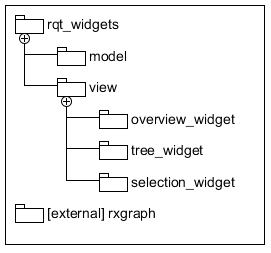
\includegraphics[scale=1.0]{./bilder/package_structure_gui.png}
\caption{The package structure of the GUI}
\label{The package structure of the GUI}
\end{center}
\end{figure}

\mbox{}

\newpage


\section{GUI - Model}
\begin{figure}[!ht]
\begin{center}
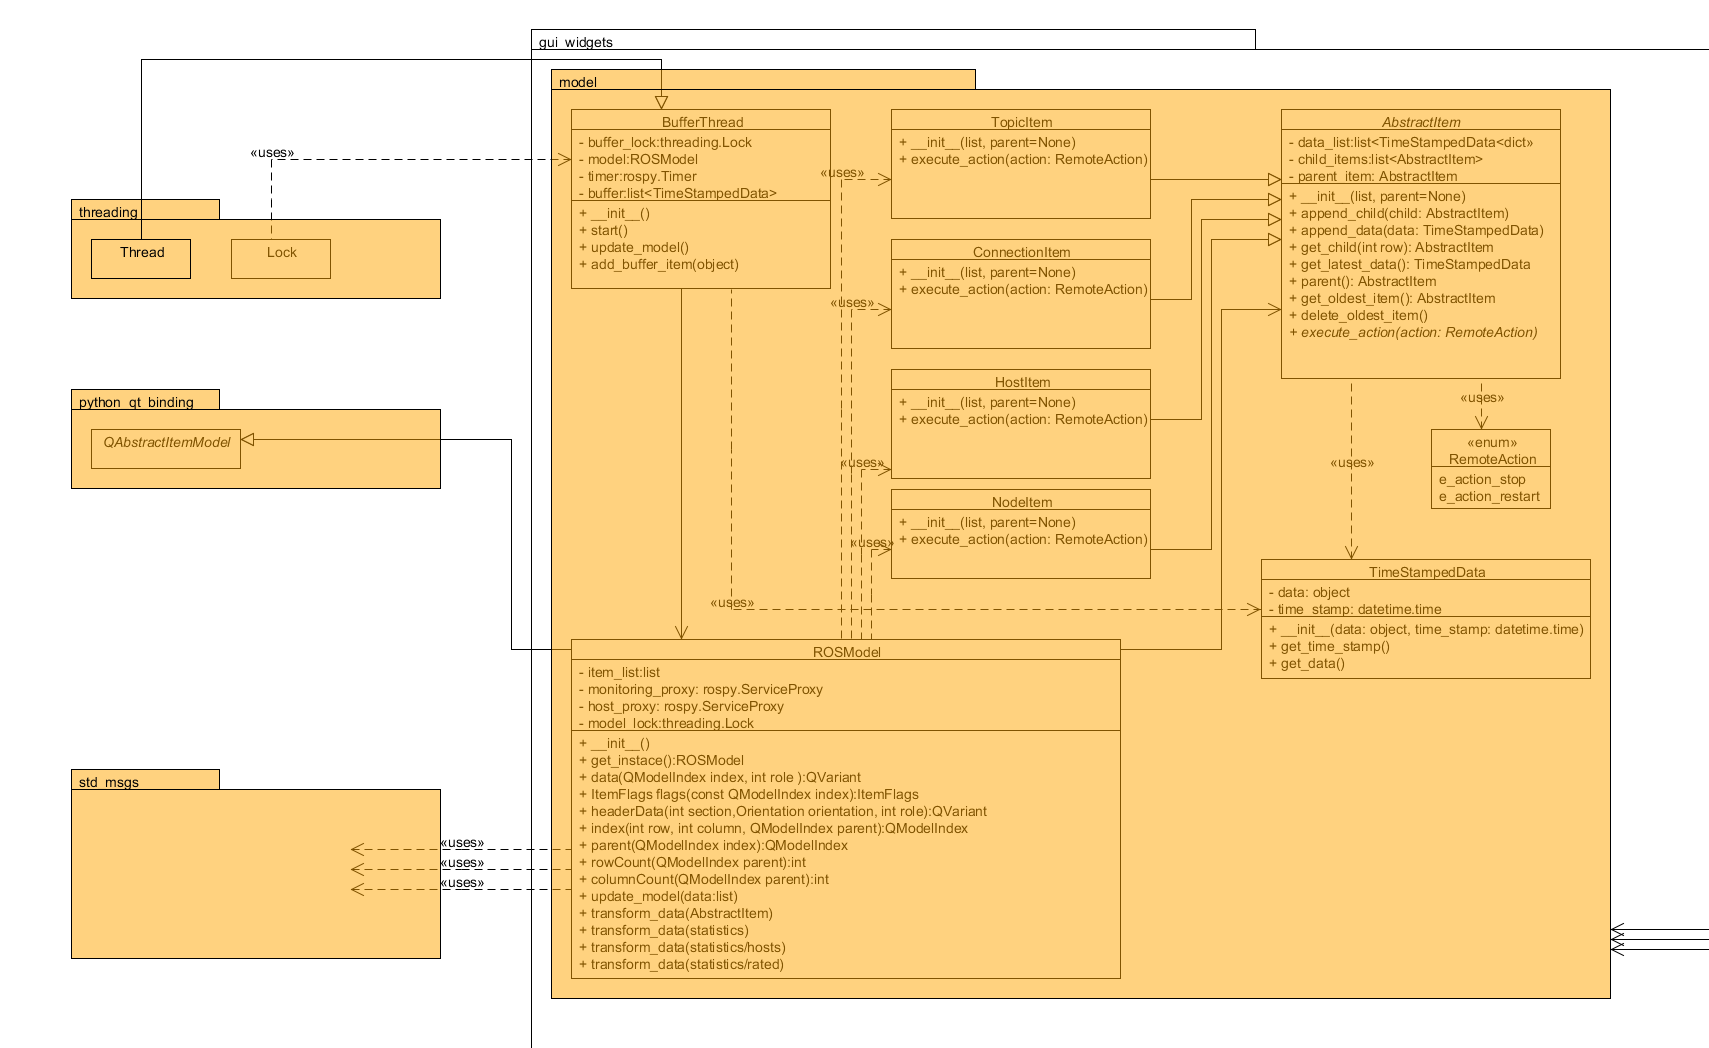
\includegraphics[width=1.0\linewidth]{./bilder/model.png}
\caption{The model class diagram}
\end{center}
\end{figure}

\subsection{BufferThread}
This thread should buffer the incoming data and regulary update the model and
hence also the model.
\subsubsection{Attributes}
\begin{itemize}
  \item private buffer\_lock: threading.Lock\\
  ..
  \item private model: ROSModel\\
  ..
  \item private timer: rospy.Timer\\
  ..
  \item private buffer: list<TimeStampedData>\\
  ..
\end{itemize}
\subsubsection{Methods}
\begin{itemize}
  \item public \_\_init\_\_()\\
  ..
  \item public start()\\
  ..
  \item public update\_model()\\
  ..
  \item public add\_buffer\_ite(object)\\
  ..
\end{itemize}

\subsection{ROSModel}
Represents the data as a QtModel. This enables automated updates of the View.
\subsubsection{Attributes}
\begin{itemize}
  \item private item\_list: list\\
  ..
  \item private monitoring\_proxy: rospy.ServiceProxy\\
  ..
  \item private host\_proxy: rospy.ServiceProxy\\
  ..  
  \item private model\_lock: threading.Lock\\
  ..
\end{itemize}
\subsubsection{Methods}
\begin{itemize}
  \item public \_\_init\_\_()\\
  ..
  \item public QVariant data(QModelIndex, int)\\
  ..
  \item public ItemFlags flags(const QModelIndex)\\
  ..
  \item public QVariant headerData(int, Orientation, int)\\
  ..
  \item public QModelIndex index(int, int, QModelIndex)\\
  ..
  \item public QModelIndex parent(QModelIndex)\\
  ..
  \item public int rowCount(QModelIndex)\\
  ..
  \item public int columnCount(QModelIndex)\\
  ..
  \item public update\_model(data:list)\\
  ..
  \item public transform\_data(AbstractItem)\\
  ..
  \item public transform\_data(statistics)\\
  ..
  \item public transform\_data(statistics/host)\\
  ..
  \item public transform\_data(statistics/rated)\\
  ..
  \end{itemize}

\subsection{AbstractItem}
Provides a unified interface to access the items of a model.
\subsubsection{Attributes}
\begin{itemize}
  \item private data\_list: list<TimeStampedData>\\
  ..
  \item private child\_items: list<AbstractItem>\\
  ..
  \item private parent\_item: AbstractItem\\
  ..
\end{itemize}
\subsubsection{Methods}
\begin{itemize}
  \item public \_\_init(list, parent=None)\_\_\\
  ..
  \item public append\_child(AbstractItem)\\
  ..
  \item public append\_data(TimeStampedData)\\
  ..
  \item public AbstractItem get\_child(int)\\
  ..
  \item public TimeStampedData get\_latest\_data()\\
  ..
  \item public AbstractItem parent()\\
  ..
  \item public AbstractItem get\_oldest\_item()\\
  ..
  \item public delete\_oldest\_item()\\
  ..
  \item public abstract execute\_action(RemoteAction)\\
  ..  
\end{itemize}

\subsection{HostItem}
A HostItem represents a host with all its data.
\subsubsection{Methods}
\begin{itemize}
  \item public \_\_init(list, parent=None)\_\_\\
  ..
  \item public execute\_action(RemoteAction)\\
  ..
\end{itemize}

\subsection{NodeItem}
 A NodeItem represents a node with all of its data. It also has a interface to start/stop/restart nodes.
\subsubsection{Methods}
\begin{itemize}
  \item public \_\_init(list, parent=None)\_\_\\
  ..
  \item public execute\_action(RemoteAction)\\
  ..
\end{itemize}

\subsection{TopicItem}
..
\subsubsection{Methods}
\begin{itemize}
  \item public \_\_init(list, parent=None)\_\_\\
  ..
  \item public execute\_action(RemoteAction)\\
  ..
\end{itemize}

\subsection{ConnectionItem}
 A NodeItem represents a node with all of its data. It also has a interface to start/stop/restart nodes.
\subsubsection{Methods}
\begin{itemize}
  \item public \_\_init(list, parent=None)\_\_\\
  ..
  \item public execute\_action(RemoteAction)\\
  ..
\end{itemize}

\subsection{TimeStampedData}
..
\subsubsection{Attributes}
\begin{itemize}
  \item private data: object\\
  ..
  \item private time\_stamp: datetime.time\\
  ..
\end{itemize}
\subsubsection{Methods}
\begin{itemize}
  \item public \_\_init(object, datetime.time)\_\_\\
  ..
  \item public datetime.time get\_time\_stamp()\\
  ..
  \item public object get\_data()\\
  ..
\end{itemize}

\subsection{Enum RemoteAction}
TODO: Description
\subsubsection{Types}
\begin{itemize}
	\item e\_action\_stop\\
	..
	\item e\_action\_restart\\
	..
\end{itemize}

\section{GUI - View}
\begin{figure}[!ht]
\begin{center}
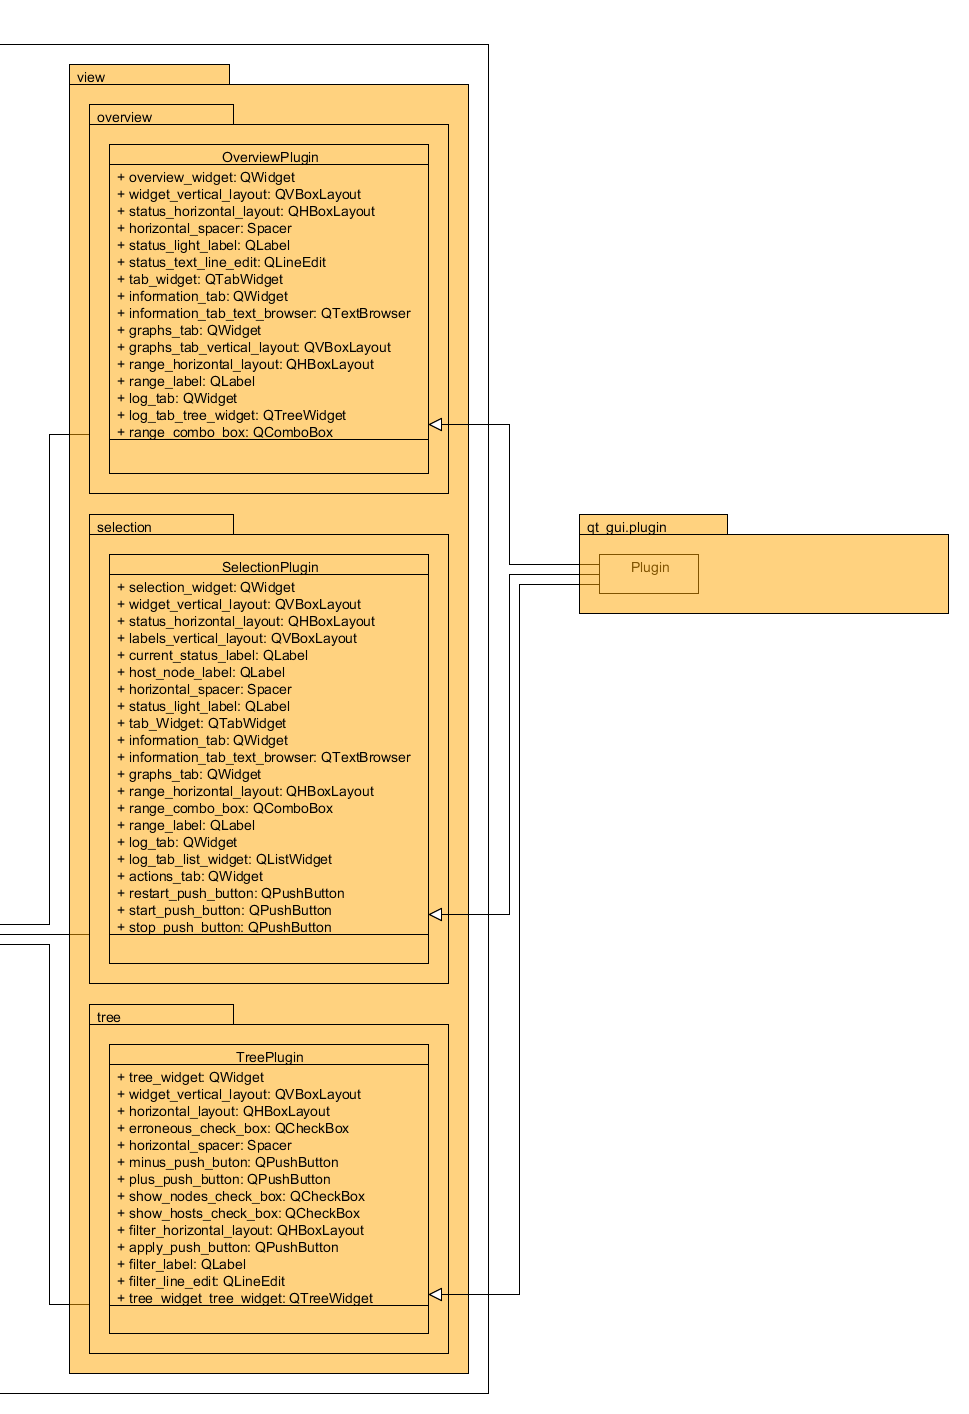
\includegraphics[width=\linewidth]{./bilder/view.png}
\caption{The view class diagram}
\end{center}
\end{figure}

\subsection{OverviewPlugin}
The class OverviewPlugin is the core of the graphical user interface, which
contains most of the relevant information in a small and fancy area.
\subsubsection{Attributes}
\begin{itemize}
  \item public overview\_widget: QWidget\\
  the object wich holds the widget
  \item public status\_light\_label: QLabel\\
  shows the actual status of the host/node
  \item public tab\_widget: QTabWidget\\
  the object wich holds the different tabs of the widget
  \item public information\_tab: QWidget\\
  a tab wich gives general information about the network 
  \item public graphs\_tab: QWidget\\
  shows the actual Network- and CPU-Load
  \item public range\_combo\_box: QComboBox\\
  makes it possible to set the range of the graphs
  \item public log\_tab: QWidget\\
  shows actual errors and warnings
  \item public log\_tab\_tree\_widget: QTreeWidget\\
  the structure of the log-messages  
\end{itemize}

\subsection{SelectionPlugin}
A class which shows detailed information in a Tree-Layout about the currently
selected host or node.
\subsubsection{Attributes}
\begin{itemize}
  \item public selection\_widget: QWidget\\
  the object wich holds the widget
  \item public host\_node\_label: QLabel\\
  shows the name of the actual selected host or node
  \item public status\_light\_label: QLabel\\
  shows the status of the host or node
  \item public tab\_widget: QTabWidget\\
  the object wich holds the different tabs of the widget
  \item public information\_tab: QWidget\\
  a tab wich gives general information about host or node 
  \item public graphs\_tab: QWidget\\
  shows the actual Network- and CPU-Load
  \item public range\_combo\_box: QComboBox\\
  makes it possible to set the range of the graphs
  \item public log\_tab: QWidget\\
  shows actual errors and warnings
  \item public actions\_tab: QWidget\\
  includes buttons to start/restart/stop nodes
  
\end{itemize}

\subsection{TreePlugin}
TreePlugin is very simply and shows only the actual active hosts
and nodes.
\subsubsection{Attributes}
\begin{itemize}
  \item public tree\_widget: QWidget\\
  the object wich holds the widget
  \item public erroneous\_check\_box: QCheckBox\\
  displays only erroneous hosts and nodes
  \item public show\_node\_check\_box: QCheckBox\\
  displays nodes
  \item public show\_host\_check\_box: QCheckBox\\
  ..hosts
  \item public minus\_push\_button: QPushButton\\
  makes it possible to zoom out
  \item public plus\_push\_button: QPushButton\\
  ..zoom in
  \item public filter\_line\_edit: QLineEdit\\
  a textfield where you can filter the output
\end{itemize}

